	\begin{frame}
		\frametitle{Motivation and principles of compressive learning}
		
		\begin{block}{What is the setup?}
			We are confronted with a dataset which comes in form of $n$ d-dimensional vectors {$\{x_{i}\}_{i = 1}^{n}$}. We would like to perform some kind of learning on it but we are scared of the complexity when $n$ is huge.
			
		\end{block}
		
		\begin{block}{What is compressive learning?}
			The principle of compressive learning consists of compressing (sketching) the dataset before applying any learning techniques. The sketch consists of a single vector $\tilde{z}$ which is constructed by transforming each vector of the dataset and averaging the results :
			$$
			\tilde{z} = \frac{1}{n}\sum_{i = 1}^{n} \Phi(x_{i})
			$$
		\end{block}
	\end{frame}
	
	\begin{frame}
		\frametitle{Motivation and principles of compressive learning}
		
		\begin{table}
			\begin{tabular}{c | c | c | c }
				$x_{1}$ & $x_{2}$ & \ldots & $x_{n}$ \\
				\hline \hline
				$x_{11}$ & $x_{12}$ & \ldots & $x_{1n}$  \\ 
				$x_{21}$  & $x_{22}$ & \ldots & $x_{2n}$\\
				\vdots & \vdots & \ldots & \vdots\\
				$x_{d1}$ & $x_{d2}$ & \ldots & $x_{dn}$
			\end{tabular}
			\caption{Initial dataset}
		\end{table}
		\resizebox{\textwidth}{!}{%
		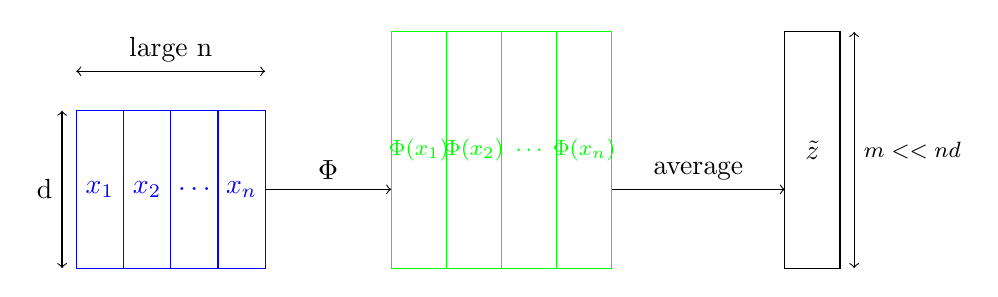
\begin{tikzpicture}
			\draw[<->] (0,2.5) -- (2.4,2.5) node[midway, above] {large n};
			\draw[<->] (-0.18, 2) -- (-0.18, 0) node[midway, left] {d};
			\draw[blue] (0, 0) rectangle (0.6, 2) node [pos = .5] {$x_{1}$};
			\draw[blue] (0.6, 0) rectangle (1.2, 2) node [pos = .5] {$x_{2}$};
			\draw[blue] (1.2, 0) rectangle (1.8, 2) node [pos = .5] {$\ldots$};
			\draw[blue] (1.8, 0) rectangle (2.4, 2) node [pos = .5] {$x_{n}$};
			
			\draw[->] (2.4,1) -- (4,1) node[midway, above] {$\Phi$};
			
			\draw[green] (4, 0) rectangle (4.7, 3) node [pos = .5] {{\footnotesize $ \Phi(x_{1})$ }};
			\draw[green] (4.7, 0) rectangle (5.4, 3) node [pos = .5] {\footnotesize{$\Phi(x_{2})$}};
			\draw[green] (5.4, 0) rectangle (6.1, 3) node [pos = .5] {\footnotesize$\ldots$};
			\draw[green] (6.1, 0) rectangle (6.8, 3) node [pos = .5] {\footnotesize$\Phi(x_{n})$};
			
			\draw[->] (6.8,1) -- (9,1) node[midway, above] {average};
			
			\draw[black] (9, 0) rectangle (9.7, 3) node [pos = .5]{$\tilde{z}$};
			\draw[<->] (9.88, 0) -- (9.88, 3) node[midway, right] {\footnotesize$m << nd$};
			
		\end{tikzpicture}
	}
	\end{frame}
	
	